\documentclass[a4paper,11pt]{report}

\usepackage{graphicx}
\usepackage{color}

\setlength{\parskip}{\baselineskip}%
\setlength{\parindent}{0pt}%

\begin{document}



\chapter{What's TIC.}


\paragraph{The language of ICT: Information and communication technology\\
\textit{Tim Shortis}\\
Psychology Press, 2001\\
The Language of \textbf{ICT}: explores the nature of the electronic word and presents the new types of text in which it is found, examines the impact of the rapid technological change we are living through, analyses different texts, including email and answerphone messages, webpages, faxes, computer games and articles about \textbf{IT} provides detailed guidance on downloading material from the web, gives URLs to visit, and includes a dedicated webpage includes a comprehensive glossary of terms.} source: google scholar

\begin{figure} [!h]
\centering
 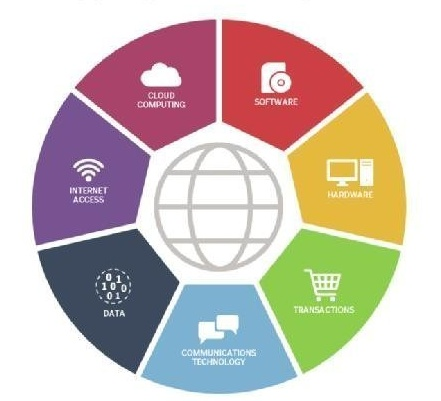
\includegraphics[scale=0.2]{tic.jpeg}
\end{figure}
\paragraph{ICT is also used to refer to the convergence of audiovisuals and telephone networks with computer networks through a single cabling or link system.}




\chapter{How to use TIC.}
\paragraph{To use the technology of information and communication, you should be connected to certain services that provide you to get the maximum benefit from the community, and getting information as smooth as possible.}

\paragraph{the table below show some of the products that is related to TIC} 


\begin{center}
\begin{tabular}{|c|c|c|}
\hline
     searching & creating & communicating \\
     \hline
     google engines & office  &  git  \\
     \hline
     google scholar & visual studio  &  meet \\
     \hline
     microsoft edge &  latex  & discord  \\
     \hline
     
\end{tabular}
\end{center}
\clearpage
\begin{figure}
    \centering
    
\includegraphics[scale=0.3]{img2.png}
\end{figure}
\section{google.}
\paragraph{Google LLC is an American multinational technology company focusing on artificial intelligence, online advertising, search engine technology, cloud computing, computer software, quantum computing, e-commerce, and consumer electronics.}source:wikipedia
\subsection{google products.}

\begin{itemize}
    \item Google Search
    \begin{itemize}
        \item Google Search (also known simply as Google or Google.com) is a search engine owned and operated by Google.
    \end{itemize}
\end{itemize}


\begin{itemize}
    \item Google Scholar
    \begin{itemize}
        \item Google Scholar is a freely accessible web search engine that indexes the full text or metadata of scholarly literature across an array of publishing formats and disciplines.
    \end{itemize}
\end{itemize}

\begin{itemize}
    \item Google Meet
    \begin{itemize}
        \item Google Meet is a video communication service developed by Google. It is one of two apps that constitute the replacement for Google Hangouts, the other being Google Chat.
    \end{itemize}
\end{itemize}
\begin{figure}[!h]
\centering
      
\includegraphics[scale=0.2]{img3.png}
      \hspace{1cm}
      
\includegraphics[scale=0.3]{img4.png}
      \hspace{1cm}
      
\includegraphics[scale=0.2]{img5.png}
\end{figure}



\clearpage

\begin{figure}
    \centering
    
\includegraphics[scale=0.5]{img6.png}
    
\end{figure}

\section{microsoft.}

    \paragraph{Microsoft Corporation is an American multinational technology corporation headquartered in Redmond, Washington.}source:wikipedia

\subsection{microsoft products.}
\begin{itemize}
    \item Windows
    \begin{itemize}
         \item Microsoft Windows is a group of several proprietary graphical operating system families developed and marketed by Microsoft.\\
         Windows is the most popular desktop operating system in the world, with a 70(persent) market share as of March 2023, according to StatCounter.
\end{itemize}
\end{itemize}

\begin{center}
    

\begin{tabular}{|c|c|}
\hline
   windows version  & year   \\ 
   \hline
    windows xp &2001 \\
     \hline
   windows vista &2007 \\
     \hline
    windows 7&2009 \\
     \hline
    windows 8&2012  \\
     \hline
   windows  10&2015 \\
    \hline
   windows 11&2021  \\
    \hline
\end{tabular}
\end{center}
\begin{figure}[!h]
    \centering
    
\includegraphics[scale=0.4]{img7.png}
    
    
\end{figure}

\clearpage
\begin{itemize}
    \item Office
    \begin{itemize}
         \item Microsoft Office, or simply Office, is a family of client software, server software, and services developed by Microsoft.\\
         It contains a word processor (Word), a spreadsheet program (Excel) and a presentation program (PowerPoint), an email client (Outlook), a database management system (Access), and a desktop publishing app (Publisher).
\end{itemize}
\end{itemize}
\begin{center}
\begin{tabular}{|c|c|}

\hline
  Office version   & year \\
     \hline
   Office 2007  &  January 30, 2007\\
     \hline
    Office 2016 & September 22, 2015  \\
     \hline
   Office 2021 & October 5, 2021 \\
   \hline
\end{tabular}
\end{center}
\begin{itemize}
    \item Visual Studio
    \begin{itemize}
        \item Visual Studio is an integrated development environment (IDE) from Microsoft. It is used to develop computer programs including websites, web apps, web services and mobile apps.\\
        Visual Studio includes a code editor supporting IntelliSense (the code completion component) as well as code refactoring.
\end{itemize}
\end{itemize}
\begin{figure}[!h]
    \centering
    
    
\includegraphics[scale=0.9]{img8.png}
    \hspace{1cm}
    
\includegraphics[scale=0.25]{img9.png}
    
\end{figure}

\clearpage
\section{Git.}
\paragraph{Git was originally authored by \textit{Linus Torvalds} in 2005 for development of the Linux kernel, with other kernel developers contributing to its initial development.\\Git is a distributed version control system that tracks changes in any set of computer files, usually used for coordinating work among programmers who are collaboratively developing source code during software development.}
\hspace {1cm}
source:wikipedia

    \begin{figure}[!h]
    \centering
    
\includegraphics[scale=0.3]{img10.png}
\end{figure}



\subsection{products that use Git.}
\begin{itemize}
    \item GitHub
    \begin{itemize}
         \item GitHub, Inc. Is an AI-powered developer platform that allows developers to create, store, and manage their code. It uses Git software, providing the distributed version control of Git plus access control, bug tracking, software feature requests, task management, continuous integration, and wikis for every project.
\end{itemize}
\end{itemize}

\begin{itemize}
    \item CRED
    \begin{itemize}
         \item CRED is an Indian fintech company. It is based in Bangalore. Founded in 2018 by \textit{Kunal Shah}, it is a reward-based credit card payments app.As of April 2021, Cred offered six different products; Cred RentPay, Cred Cash, Cred Pay, Cred Store, and Cred Travel Store, etc.
\end{itemize}
\end{itemize}



\begin{figure}[!h]
    \centering
    
\includegraphics[scale=0.01]{img11.png}
    \hspace{3cm}

\includegraphics[scale=0.2]{img12.png}
\end{figure}

\clearpage

\section{Websites providing online usage.}
\subsection{Replit.}

\paragraph{Replit is an online IDE website, provides access for multiple coding editors, such as python, js, c, ect. The site has many extra services like AI and forking. Forking in replit means sharing code, because when you write a code the site will automatic set it on your personnel profil page, and any one can click on fork button to copy the cod to his editor.}personnel experience
\paragraph{Replit was co-founded by programmers \textit{Amjad Masad}, \textit{Faris Masad}, and designer Haya Odeh in 2016.}source:wikipedia
\begin{figure}[!h]
    \centering
    
\includegraphics[scale=0.1]{img13.png}
    
\end{figure}

\subsubsection{Some of the languages that replit supports.}

\begin{itemize}
    \item C
    \begin{itemize}
         \item C is a general purpose programming languages, powered by a compiler. The compiler is translator, that translate the programming language to the machine language. The compiler translate the code completely , after organizing it.
\end{itemize}
\end{itemize}
\begin{itemize}
    \item Python
    \begin{itemize}
        \item python is a general purpose programming, powered by an interpreter. The interpreter is like the compiler, but he translate the code line by line.
\end{itemize}
\end{itemize}
\begin{figure}[!h]
    \centering
    
\includegraphics[scale=0.075]{img14.png}
    \hspace{3cm}
    
\includegraphics[scale=0.5]{img15.jpeg}
    
\end{figure}
\clearpage
\subsection{Overleaf.}
\paragraph{Overleaf is an online web site, provides a complete LaTex usage. The site have lots of templates, it makes the experience faster for beginners.}personnel experience
\paragraph{It partners with a wide range of scientific publishers to provide official journal LaTeX templates, and direct submission links.} source:\\wikipidea
\begin{itemize}
    \item LaTex
    \begin{itemize}
        \item LaTex is a pdf logiciel that uses commands to write the code on the editor, and a compiler to translate the code to a high quality pdf.
        
        
\end{itemize}
    \begin{itemize}
            \item LaTeX was created in the early 1980s by \textit{Leslie Lamport} when he was working at SRI.
        \end{itemize}
            
\end{itemize}
    
\begin{figure}[!h]
    \centering
    
\includegraphics[scale=0.2]{img16.png}
    \hfill
    
\includegraphics[scale=0.15]{img17.png}
\end{figure}
Some Latex commands:\\
\begin{centering}
\begin{tabular}{|c|c|}

\hline
    command & fonction \\
\hline
  begin ... end& environment\\
\hline
section,subsection&titles\\
\hline
itemze &item environment\\
\hline
tabular&table environment\\
\hline
hspace&space between elements\\
\hline
hline&horizon line\\
\hline



\end{tabular}

\end{centering}
note: all commands starts with back slash.

\clearpage

\centering {\Large{Index}}

\begin{enumerate}
    \item \large{\textcolor{red}{What's TIC.}}


    \item \large{\textcolor{red}{How to use TIC.}}
    \begin{enumerate}
        \item Google.
                \begin{itemize}
                    \item Google products.
                         \begin{itemize}
                             \item Google Search
                             \item Google Scholar
                             \item Google Meet
                             
                         \end{itemize}
                \end{itemize}
        \item microsoft.
                     \begin{itemize}
                         \item Microsoft products.
                         \begin{itemize}
                             \item Windows
                             \item Office
                             \item Visual Studio
                             
                         \end{itemize}
                     \end{itemize}
        \item Git.
                 \begin{itemize}
                     \item Products that use get.
                     \begin{itemize}
                             \item GitHub
                             \item Cred
                             
                             
                         \end{itemize}
                 \end{itemize}
        \item Websits providing online usage.
             \begin{itemize}
                 \item Replit.
                 \begin{itemize}
                 \item Some of the languages that replit support
                 \begin{itemize}
                             \item C
                             \item Python
                         \end{itemize}
                         \end{itemize}
                 \item Overleaf.
                 \begin{itemize}
                             \item LaTex
                             
                         \end{itemize}
             \end{itemize}
\end{enumerate}
\end{enumerate}



\end{document}
